% Tikz flowchart to show passage history for JEV vaccine strain

%block styles for the chart.
\tikzstyle{parent} = [rectangle, draw, fill=red!20, 
minimum width=7.2em, text badly centered, node distance=1cm, minimum height=1.2em, inner sep=0pt]
\tikzstyle{intermediate} = [rectangle, draw, fill=blue!20, 
minimum width=7.2em,text badly centered, node distance=1cm, minimum height=1.2em, inner sep=0pt]
\tikzstyle{information} = [rectangle, draw, fill=white, 
minimum width=7.2em, text badly centered, node distance=3cm, minimum height=1.2em,inner sep=0pt]
\tikzstyle{studied} = [rectangle, draw, fill=yellow, 
minimum width=7.2em, text badly centered, node distance=1cm, minimum height=1.2em,inner sep=0pt]
\tikzstyle{line} = [draw]
\tikzstyle{arrow} = [thick,->,>=stealth,draw]
%\tikzstyle{dashed} = [thick,dashed,draw]

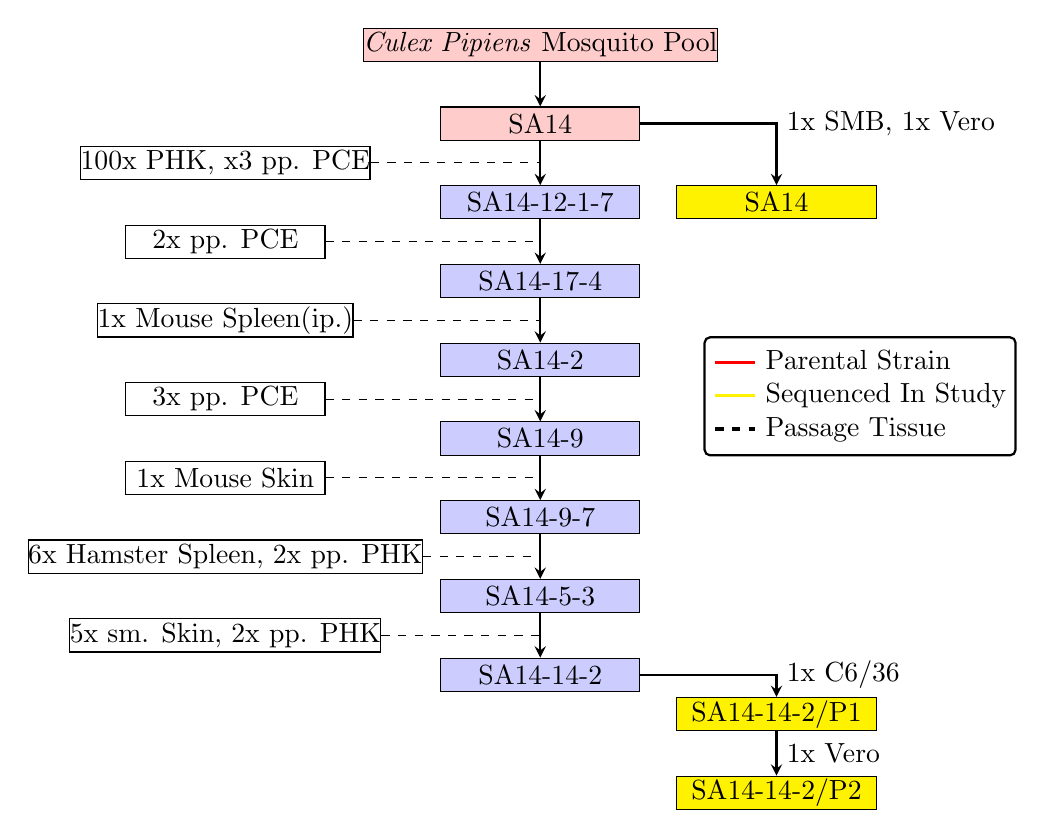
\begin{tikzpicture}[auto]

%\draw[help lines,step=.5] (0,0) grid (12,12);

	%Nodes for each of the strains mentioned by Yu 2010
	\node[parent](Mosquito) at (6,12) {\emph{Culex Pipiens} Mosquito Pool};
	\node[parent, below of=Mosquito](SA14){SA14};
	\node[intermediate, below of=SA14](SA14-12-1-7){SA14-12-1-7};
	\node[intermediate, below of=SA14-12-1-7](SA14-17-4){SA14-17-4};
	\node[intermediate, below of=SA14-17-4](SA14-2){SA14-2};
	\node[intermediate, below of=SA14-2](SA14-9){SA14-9};
	\node[intermediate, below of=SA14-9](SA14-9-7){SA14-9-7};
	\node[intermediate, below of=SA14-9-7](SA14-5-3){SA14-5-3};
	\node[intermediate, below of=SA14-5-3](SA14-14-2){SA14-14-2};
%	\node[intermediate, below of=SA14-14-2](SA14-14-2-PDK){SA14-14-2 PDK};
	
	%Nodes for each of the three strains considered in the study.
	\node[studied](TYF2350) at ([xshift=3cm,yshift=-1cm]SA14) {SA14};
	\node[studied](TYF1454)at ([xshift=3cm,yshift=-0.5cm]SA14-14-2){SA14-14-2/P1};
	\node[studied, below of=TYF1454](TYF1910){SA14-14-2/P2};	

	%Arrows connecting the three strains considered in the study.
	\path[arrow] (SA14-14-2) -| node {1x C6/36}(TYF1454);
	\path[arrow] (TYF1454) -- node {1x Vero} (TYF1910);
	\path[arrow] (SA14) -| node{1x SMB, 1x Vero} (TYF2350);
	
	%Arrow connecting Paths
	\path[arrow] (Mosquito) -- coordinate[midway](M1) (SA14);
	\path[arrow] (SA14) -- coordinate[midway](M2) (SA14-12-1-7);
	\path[arrow] (SA14-12-1-7) -- coordinate[midway](M3) (SA14-17-4);
	\path[arrow] (SA14-17-4) -- coordinate[midway](M4) (SA14-2);
	\path[arrow] (SA14-2) -- coordinate[midway](M5) (SA14-9);
	\path[arrow] (SA14-9) -- coordinate[midway](M6) (SA14-9-7);
	\path[arrow] (SA14-9-7) -- coordinate[midway](M7) (SA14-5-3);
	\path[arrow] (SA14-5-3) -- coordinate[midway](M8) (SA14-14-2);
%	\path[arrow] (SA14-14-2) -- coordinate[midway](M9) (SA14-14-2-PDK);

	%Nodes for the passage information
%	\node[information](Mosquito_pass) at ([xshift=-4cm]M1) {11x mb.};
	\node[information](SA14_pass) at ([xshift=-4cm]M2) {100x PHK, x3 pp. PCE};
	\node[information](SA14-12-1-7_pass) at ([xshift=-4cm]M3) {2x pp. PCE};
	\node[information](SA14-17-4_pass) at ([xshift=-4cm]M4) {1x Mouse Spleen(ip.)};
	\node[information](SA14-2_pass) at ([xshift=-4cm]M5) {3x pp. PCE};
	\node[information](SA14-9_pass) at ([xshift=-4cm]M6) {1x Mouse Skin};
	\node[information](SA14-9-7_pass) at ([xshift=-4cm]M7) {6x Hamster Spleen, 2x pp. PHK};
	\node[information](SA14-5-3_pass) at ([xshift=-4cm]M8) {5x sm. Skin, 2x pp. PHK};
%	\node[information](SA14-14-2_pass) at ([xshift=-4cm]M9) {9x PDK};

	%Paths connecting passage information nodes with center of arrows.
%	\path[line,dashed] (Mosquito_pass) -- (M1);	
	\path[line,dashed] (SA14_pass) -- (M2);	
	\path[line,dashed] (SA14-12-1-7_pass) -- (M3);	
	\path[line,dashed] (SA14-17-4_pass) -- (M4);
	\path[line,dashed] (SA14-2_pass) -- (M5);	
	\path[line,dashed] (SA14-9_pass) -- (M6);	
	\path[line,dashed] (SA14-9-7_pass) -- (M7);	
	\path[line,dashed] (SA14-5-3_pass) -- (M8);	
%	\path[line,dashed] (SA14-14-2_pass) -- (M9);	

					
	\node[draw=black,thick,rounded corners=2pt,below left=2mm] at (12.25,8.5) {%
		\begin{tabular}{@{}r@{ }l@{}}
		%	\raisebox{2pt}{\tikz{\draw[gray, very thick, dashed] (0,0) -- (5mm,0);}}&National Origin\\
		\raisebox{2pt}{\tikz{\draw[red, very thick] (0,0) -- (5mm,0);}}&Parental Strain\\
		\raisebox{2pt}{\tikz{\draw[yellow, very thick] (0,0) -- (5mm,0);}}&Sequenced In Study\\
		\raisebox{2pt}{\tikz{\draw[black,dashed, very thick] (0,0) -- (5mm,0);}}&Passage Tissue\\
		\end{tabular}};
\end{tikzpicture}